\section{DESENVOLVIMENTO}

\subsection{Introdução ao Eureka}

Neste trabalho tem-se por objetivo o a pesquisa e desenvolvimento de uma estrutura IoT baseado no padrão de micro-serviços, e para isto precisa-se utilizar um dos princípios que foi citada na revisão bibliográfica que é o "Service Discovery" ou descoberta de serviços. Como o projeto será baseado em Java, inicialmente será criado um projeto e  utilizará maven para gerenciamento de dependências e o Eureka Client para descoberta de serviços. Para poder utilizar o maven deve-se criar um arquivo de configurações no diretório raíz do projeto chamado "pom.xml", e a documentação completa pode se encontrar no site de seus desenvolvedor. Posteriormente será incluso o seguinte groupId org.springframework.cloud e o artifactId spring-cloud-starter-eureka, e para mais informações pode ser encontrada na documentação oficial do Spring Cloud Netflix.

Quando um cliente se registra com o Eureka, ele fornece meta-dados sobre si, indicador de estado ou saúde, página inicial, dentre outros. Eureka recebe mensagens heartbeat (disponibilidade) de cada instância pertencente a um serviço. Se algum heartbeat falhar, a instância é removido do registro.
Para inicializar um projeto com Eureka Client, será utilizado algumas anotações Java fornecidas pelo Eureka descritas a seguir: @Configuration, para utilizar recursos do projeto Spring Config para facilitar configurações de projetos Spring baseado em Java, @ComponentScan para buscar componentes em pacotes java, @EnableAutoConfiguration para ativar a ComponentScandescritas a seguir: @EnableEurekaClient para ativar a descoberta de serviços do Eureka, @RestController para criar um controlador Rest (Representational State Transfer), @RequestMapping para mapear as rotas da aplicação.

\begin{verbatim}
@Configuration
@ComponentScan
@EnableAutoConfiguration
@EnableEurekaClient
@RestController
public class Application {

    @RequestMapping("/")
    public String home() {
        return "Hello world";
    }

    public static void main(String[] args) {
        new SpringApplicationBuilder(Application.class)
          .web(true).run(args);
    }
}
\end{verbatim}

Para que possa surtir efeito na aplicação precisa fazer ajustes nas configurações do Eureka dentro do diretório resources da aplicação Java. Esta configuração é feita dentro de um arquivo Application.yml.

\begin{verbatim}
  Eureka
   cliente:
     ServiceUrl:
       DefaultZone: http: // localhost: 8761 / eureka / 
\end{verbatim}

Neste arquivo de configuração encontra-se uma peculariedade. O DefaultZone é a URL do serviço Eureka para qualquer cliente. O nome do aplicativo padrão (ID de serviço), o host e a porta podem ser acessadas respectivamente pelas variáveis de ambientes: \${spring.application.name} , \${spring.application.name} e \${server.port}.
A anotação Java @EnableEurekaClient faz com que o a aplicação corrente se registre no Eureka, para que assim possa localizar outros serviços.

\subsection{Status e Saúde do serviço}

Com a página de status e os indicadores de integridade de uma instância do Eureka é possível visualizar informações do serviço. Para acessar os indicadores de saúde deve-se configurar as rotas padrões de acesso a mesma. Por padrão, o eureka utiliza a conexão do cliente para determinar se um cliente está ativo. Caso não utilize o Discovery Client, não será propagado o status de verificação de integridade atual do serviço. Para funcionar corretamente os indicadores de saúde e status da aplicação, devem ser feitas as seguintes configurações:

\begin{verbatim}
eureka:
  instance:
    statusPageUrlPath: ${management.context-path}/info
    healthCheckUrlPath: ${management.context-path}/health
  client:
    healthcheck:
      enabled: true
\end{verbatim}

Para conseguir utilizar mais recursos e obter mais informações sobre o status da aplicação, a aplicação deve implementar seu próprio controle de integridade que se encontra no pacote com.netflix.appinfo.HealthCheckHandler

\subsection{Alterando o ID da instância Eureka}

Uma instancia registrada no Eureka possui seu ID, que identifica o serviço que está no mesmo. O Spring Cloud Eureka fornece o seguinte padrão de configuração: \$\{spring.cloud.client.hostname\}:\$\{spring.application.name\}:\$\{spring.application.instance\_id:
\$\{server.port\}\}. Como exemplo a URL fica da seguinte maneira: myhost:myapp:8080

\subsection{EurekaClient}

O próximo passo para aprender a utilizar os clientes Eureka, é aprende a utlizar o EurekaClient, que pode ser utilizado para descobrir instâncias do Eureka Server. Para fazer isto utilizando o framework desenvolvido para Java pela Spring Cloud, precisa primeiramente injetar a dependência do EurekaClient e criar um método que busque as instâncias registradas no Eureka.

\begin{verbatim}
@Autowired
private EurekaClient discoveryClient;

public String serviceUrl() {
    InstanceInfo instance = 
      discoveryClient.getNextServerFromEureka("STORES", false);
    return instance.getHomePageUrl();
}
\end{verbatim}

Não necessariamente precisa utilizar o EurekaClient. Também pode-se utilizar o DiscoveryClient. A diferença entre os dois, está na maneira de como é utilizado.

\begin{verbatim}
@Autowired
private DiscoveryClient discoveryClient;

public String serviceUrl() {
    List<ServiceInstance> list = 
      discoveryClient.getInstances("STORES");
    if (list != null && list.size() > 0 ) {
        return list.get(0).getUri();
    }
    return null;
}
\end{verbatim}

\subsection{Performanece de registro no Eureka}

Registrar um serviço no Eureka pode ser considerado um pouco lento, pelo fato de que ser uma instância também envolve um heartbeat periódico para o registro com duração padrão de 30 segundos. Um serviço não estará disponível para descoberta por clientes enquanto uma intância tenha todos os metadados em seu cache local. Para alterar o período em que isto ocorre pode ser configurado através da propriedade eureka.instance.leaseRenewalIntervalInSeconds. Entretanto, em produção, não deve ser alterado este padrão pelo fato de que, existem alguns cálculos internos do Eurela que fazem suposições de renovação de locação.

\subsection{Zonas Eureka}

Primeiramente, para se configurar uma zona Eureka, precisa-se ter certeza de que existem servidores Eureka implantados em cada zona e que eles são pares uns dos outros. Em seguida, precisa-se informar em qual zona o mesmo está. Para fazer isto será utilizado a propriedade metadataMap. E isto pode ser feito da seguinte forma:

\begin{verbatim}
eureka.instance.metadataMap.zone = zone1
eureka.client.preferSameZoneEureka = true
\end{verbatim}

\subsection{Primeiros passos com Eureka Server}

Primeiramente, para começar a utilizar o Eureka, como este projeto é baseado em Java no backend e utiliza maven como gerenciador de dependências, deve ser incluido nas mesmas a dependência com o groupId org.springframework.cloud e o artifactId spring-cloud-starter-eureka-server. Com esta dependência adicionada, será possível utilzar o Eureka Server.

Após adicionar esta dependência, deve ser criado a classe principal que se encarregará de iniciar a aplicação Eureka Server. Utilizando-se da anotação @EnableEurekaServer fornecida pelo framework e seguindo o padrão utilizado no Eureka Client para iniciar a aplicação, é possível ver um resultado. Um exemplo de código pode ser visto a seguir.

\begin{verbatim}
@SpringBootApplication
@EnableEurekaServer
public class Application {

    public static void main(String[] args) {
        new SpringApplicationBuilder(Application.class).web(true).run(args);
    }

}
\end{verbatim}

\subsection{Modo Autônomo}

A combinação entre o cliente e servidor Eureka e as pulsações para verificação de disponibilidade entre os mesmos, tornam o servidor Eureka Autônomo bastante resiliente à falha, contanto que haja algum tipo de monitoramento para mantê-lo funcionando. No modo autônomo, pode-se prefirir desativar o comportamento padrão do lado do cliente, para que ele não continue tentado alcançar seus pares caso haja falha. Para isto será feito diversas configurações como pode ser visto a seguir.


\begin{verbatim}
server:
  port: 8761

eureka:
  instance:
    hostname: localhost
  client:
    registerWithEureka: false
    fetchRegistry: false
    serviceUrl:
      defaultZone: http://${eureka.instance.hostname}:${server.port}/eureka/
\end{verbatim}

Com o Eureka, os registros podem ser ainda mais resistentes e disponíveis executando várias instâncias e pedindo-lhes para se registrarem uns com os outros. Tudo o que precisa para fazê-lo é configurar o serviceUrl dos pares.

\begin{verbatim}
---
spring:
  profiles: peer1
eureka:
  instance:
    hostname: peer1
  client:
    serviceUrl:
      defaultZone: http://peer2/eureka/

---
spring:
  profiles: peer2
eureka:
  instance:
    hostname: peer2
  client:
    serviceUrl:
      defaultZone: http://peer1/eureka/
\end{verbatim}

Neste exeplo, temos configurado, que o serviço pode ser utilizado para executar o mesmo servidor em 2 hosts (peer1 e peer2), executando-o em diferentes perfis Spring. Pode-se utilizar esta configuração para testar a descoberta dos pares em um único host, manipulando se em servidor Linux o arquivo hosts para resolver os nomes de host que pode ser encontrado dentro do diretório /etc/hosts.

Em alguns casos, é preferível que o Eureka utilize os endeços IP dos serviços ao invés do nome do host. Para isto deve ser definido a configuração eureka.instance.preferIpAddress como true e quando a aplicação se registrar com o Eureka, o mesmo utilizará seu endereço IP ao invés de seu nome de host.

\subsection{Clientes Hystrix}

Segundo Fowler (2016) é comum que os sistemas de software façam chamadas remotas para software em execução em diferentes processos, provavelmente em máquinas diferentes em uma rede. Uma das grandes diferenças entre chamadas em memória e chamadas remotas é que chamadas remotas podem falhar ou travar sem uma resposta até que algum limite de tempo limite seja atingido. O que é pior se você tem muitos chamadores em um fornecedor que não responde, então você pode ficar sem recursos críticos levando a falhas em cascata em vários sistemas. Em seu excelente livro Release It  , Michael Nygard popularizou o padrão de disjuntor para evitar este tipo de cascata catastrófica.

Com todos estes problemas que podem ocorrer na arquitetura de micro-serviços, a Netflix criou a biblioteca chamada Hystrix, que impelementa o padrão disjuntor que interromple automáticamente o serviço quando ocorre falhas. Uma falha de serviço no nível inferior de serviços pode causar falha em cascata em todo o caminho até o usuário. No Hystrix o padrão de limite de falhas são 20 em 5 segundos, e quando ocorre o circuito é aberto e a chamada não é feita, isto pode ser visto na figura \ref{fig:figura7}

\begin{figure}[h]
\centering
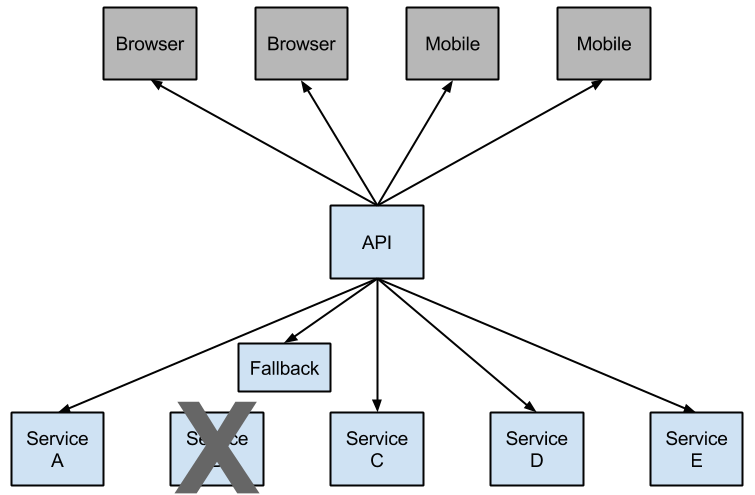
\includegraphics[height=4.2cm]{imagens/figura7}
\caption{Fallback Hystrix em falhas em cascata.}
\label{fig:figura7}
\end{figure}

\subsection{Primeiros passos com Hystrix}

Para utilizar o Hystrix, precisa seguir o mesmo padrão de quando se começa uma aplicação Eureka Server ou Client. No caso do padrão deste projeto backend baseado em Java com gerenciado de dependências maven, o que mudará será a anotação utilizada na classe principal do projeto e a dependência maven utilizada. Para incluir no projeto, será utilizado a dependência com o groupId org.springframework.cloud e o artifactId spring-cloud-starter-Hystrix, e a anotação @EnableCircuitBreaker na classe principal.

\begin{verbatim}
@SpringBootApplication
@EnableCircuitBreaker
public class Application {

    public static void main(String[] args) {
        new SpringApplicationBuilder(Application.class).web(true).run(args);
    }

}

@Component
public class StoreIntegration {

    @HystrixCommand(fallbackMethod = "defaultStores")
    public Object getStores(Map<String, Object> parameters) {
        //do stuff that might fail
    }

    public Object defaultStores(Map<String, Object> parameters) {
        return /* something useful */;
    }
}
\end{verbatim}

No exemplo de código acima, foi implementando uma classe que se contém um método que buscara os serviços, e para isto foi utilizado a anotação @HystrixCommand.

É possível ativar as métricas Hystrix e a central de gerenciamento do mesmo adicionando as dependências abaixo. O endpoint para acesso ao gerenciador é /hystrix.stream.

\begin{verbatim}
<dependency>
    <groupId>org.springframework.boot</groupId>
    <artifactId>spring-boot-starter-actuator</artifactId>
</dependency>
<dependency>
    <groupId>org.springframework.cloud</groupId>
    <artifactId>spring-cloud-starter-hystrix-dashboard</artifactId>
</dependency>
\end{verbatim}

\subsection{Ribbon}

Ribbon é um  balanceador de carga do lado do cliente que fornece controles sobre o comportamento dos clientes HTTP e TCP. Uma observação importante é que a anotação @FeignClient já utiliza Ribbon, fazendo com que assim seja desnecessário a utilização do Ribbon, entretanto, quando for preciso um controle mais versátil sobre a tecnologia é optável a utilização do mesmo.

Para incluir o ribbon no projeto, será utilizado o mesmo padrão de configurações feito anteriormente. O que será alterado é a o artifactId da dependência maven que agora será utilizado spring-cloud-starter-ribbon, e para configurar o cliente Ribbon criado uma classe de configuraçao e será anotado com @RibbonClient. 

\begin{verbatim}
@Configuration
@RibbonClient(name = "foo", configuration = FooConfiguration.class)
public class TestConfiguration {
}
\end{verbatim}

\subsection{FeignClient}

FeignClient é uma biblioteca que faz com que clientes de serviços web sejam escritos de forma mais fácil. Para utilizá-lo é preciso instalar a dependência spring-cloud-starter-feign e anotar a classe principal com @EnableFeignClients. O mesmo provê suporte para anotações Spring MVC e por utilizar o mesmo conversor de mensagens HTTP que o Spring Web, é integra com Hystrix para fornecer um cliente com balanceamento de carga.

\begin{verbatim}
@Configuration
@ComponentScan
@EnableAutoConfiguration
@EnableEurekaClient
@EnableFeignClients
public class Application {

    public static void main(String[] args) {
        SpringApplication.run(Application.class, args);
    }

}
\end{verbatim}

Ao anotar uma interface com @FeignClient, pode ser mapeado os métodos para que consiga acesso a endpoints da biblioteca. O nome do método será qualificado e aplicado ao contexto da aplicação, fazendo com que assim não seja implementado corpo ao método pois será apenas repassados chamadas REST.

\begin{verbatim}
@FeignClient("stores")
public interface StoreClient {
    @RequestMapping(method = RequestMethod.GET, value = "/stores")
    List<Store> getStores();

    @RequestMapping(method = RequestMethod.POST, value = "/stores/{storeId}", consumes = "application/json")
    Store update(@PathVariable("storeId") Long storeId, Store store);
}
\end{verbatim}

Cada Cliente Feign faz parte de um conjunto de componentes que trabalham juntos para comunicar-se via HTTP. O Spring Cloud permite com que se tenha controle total sobre clientes Feign declarando uma classe de configuração que implemente determinados métodos do FeignClient. Duas das possíveis configuração, sao: modificar o padrão de Contrato que o FeignClient utiliza para que assim seja personalizado o padrão de comunicação REST que o mesmo utiliza e modificar o método de autenticação do FeignClient.

\begin{verbatim}
@Configuration
public class FooConfiguration {
    @Bean
    public Contract feignContract() {
        return new feign.Contract.Default();
    }

    @Bean
    public BasicAuthRequestInterceptor basicAuthRequestInterceptor() {
        return new BasicAuthRequestInterceptor("user", "password");
    }
}
\end{verbatim}

Em alguns casos, pode ser necessário outros métodos mais especificos para que seja personalizado as configurações. Neste caso, pode-se utilizar a API Feign Builder. Abaixo está um exemplo da utilização do mesmo.

\begin{verbatim}
@Import(FeignClientsConfiguration.class)
class FooController {

	private FooClient fooClient;

	private FooClient adminClient;

    @Autowired
	public FooController(
			Decoder decoder, Encoder encoder, Client client) {
		this.fooClient = Feign.builder().client(client)
				.encoder(encoder)
				.decoder(decoder)
				.requestInterceptor(new BasicAuthRequestInterceptor("user", "user"))
				.target(FooClient.class, "http://PROD-SVC");
		this.adminClient = Feign.builder().client(client)
				.encoder(encoder)
				.decoder(decoder)
				.requestInterceptor(new BasicAuthRequestInterceptor("admin", "admin"))
				.target(FooClient.class, "http://PROD-SVC");
    }
}
\end{verbatim}

\subsection{Zuul}

Até neste capítulo, foi falado de rotas e endpoints, mas ainda não foi explorado a essencialidade de utilizar rotas. Roteamento é uma parte fundamental de uma arquitetura de micro-serviços pelo fato de que, uma uri (identificador uniforme de recursos) pode ser mapeado de acordo com sua utilidade. Como exemplo, uma uri \/api\/usuario é mapeado para o serviço de usuário, \/api\/vendas pode ser mapeado para o serviço de vendas de uma loja. Zuul é um roteador com balanceamento de carga básico. A empresa Netflix atualmente utiliza o Zuul para os seguintes desígnios: autenticação, insights teste de stress da api, Canary test que segundo Sato (2014) é uma técnica para reduzir o risco de introduzir uma nova versão de software na produção lentamente lançando a mudança para um pequeno subconjunto de usuário antes de lança-la em toda a infra-estrutura e torná-la disponível para todos, roteamento dinâmico, serviço de migração, divisão de carga, segurança, manipulação de respostas e gestão de tráfego de dados.

Para incluir o Zuul em um projeto utilizando os padrões aplicados até neste capítulo deve-se utilizar o artifactId spring-cloud-starter-zuul e para habilitá-lo, a classe principal deve ser anotada com @EnableZuulProxy, e este encaminhará chamadas locais para o serviço adequado. Para que de acordo com a rota seja chamado o serviço desejado deve ser configurado no arquivo de configurações principais application.yml, e para ignorar demais serviços utiliza-se a propriedade zuul.ignored-services. Abaixo está um exemplo da utilizaçao da mesma.

\begin{verbatim}
 zuul:
  ignoredServices: '*'
  routes:
    users: /meus-produtos/**
\end{verbatim}

Para obter um controle mais refinado sobre determinadas rotas, pode-se especificar o caminho e o serviceId.

\begin{verbatim}
 zuul:
  routes:
    users:
      path: /meus-produtos/**
      serviceId: produtos_service
\end{verbatim}

Isto significa que quando ocorrer uma chamado para a rota \"\/myusers\", o mesmo será encaminhado para o serviço \"users_service\". Se for desejável especificar uma URL para uma localização física do serviço, pode ser feito da seguinte maneira.

\begin{verbatim}
 zuul:
  routes:
    users:
      path: /produtos/**
      url: http://exemple.com/produtos_service
\end{verbatim}

As configurações de rotas feitas até o momento, não são executadas como um HystrixCommand ou balancedas com Ribbon. Para conseguir isto, deve-se especificar um serviço de rota e criar um cliente Ribbon para o serviceId. Abaixo, um exemplo de configuração para o mesmo.

\begin{verbatim}
zuul:
  routes:
    users:
      path: /meus-produtos/**
      serviceId: produtos

ribbon:
  eureka:
    enabled: false

users:
  ribbon:
    listOfServers: exemplo.com,faype.com
\end{verbatim}


